
\begin{figure}[h]
\centering
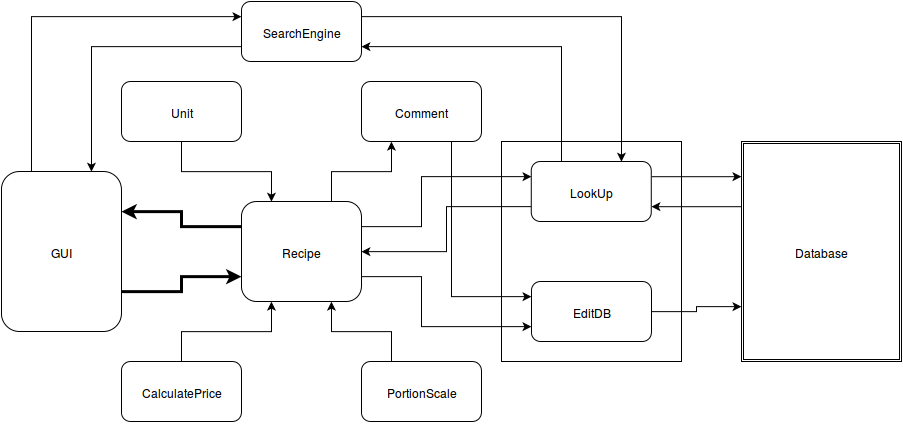
\includegraphics[scale=0.5]{overview.png}
\caption{Översikt över första lagrets moduler.}
\label{fig:overview}
\end{figure}

MatLabb har tre centrala delsystem samt en databas vilka initialt kan betraktas på följande sätt: 
\begin{enumerate}
  \item Ett användargränssnitt (\textbf{GUI}), baserat på biblioteket QT, som hjälper användaren att på ett intuitivt och välbekant sätt interagerar med receptmodulen, och i förlängningen databasen.
  \item \textbf{Shell} - ett lager som närmast kan kallas för MatLabbs styrsystem.
  \item \textbf{Lookup} - ett lager som huvudsakligen sköter kommunikationen mellan \textbf{Shell} och databasen. 
  \item En databas som lagrar all receptrelaterad information.
\end{enumerate}
I detta kapitel ges en överblick över funktionaliteten hos dessa delsystem och hur dessa interagerar.

%\section{Databas}\label{sec:ark.databas)}
Databasen utgörs av en MySQL-databas där recept, ingredienser och relaterad data lagras. Exakt data som lagras framgår i kravspecifikationen, samt i kapitel \ref{cha:tekspec} - \emph{Detaljerad teknisk specifikation}.

%\section{Shell}\label{sec:ark.shell}
\textbf{Shell} utgör det primära navet mellan databasen och användargränssnittet (\textbf{GUI}). Här behandlas aktuellt recept enligt de instruktioner som mottas via GUI:t. Modulen interagerar direkt med \textbf{GUI} och \textbf{Lookup} och indirekt med databasen via \textbf{Lookup}.

%\section{GUI}\label{sec:ark.gui}
\textbf{GUI} är en abstraktion av det grafiska användargränssnittet och i förlängningen användaren. ``Modulen'' kommunicerar med \textbf{Shell}.

%\section{Lookup}\label{sec:lookup}
\textbf{Lookup} ingår egentligen i \textbf{Shell}, men betraktat som en separat modul sköter den kommunikationen mellan databasen och \textbf{Shell}s övriga interna submoduler.
